%%%%%%%%%%%%%%%%%%%%%%%%%%%%%%%%%%%%%%%%%
% Beamer Presentation
% LaTeX Template
% Version 1.0 (10/11/12)
%
% This template has been downloaded from:
% http://www.LaTeXTemplates.com
%
% License:
% CC BY-NC-SA 3.0 (http://creativecommons.org/licenses/by-nc-sa/3.0/)
%
%%%%%%%%%%%%%%%%%%%%%%%%%%%%%%%%%%%%%%%%%

%----------------------------------------------------------------------------------------
%	PACKAGES AND THEMES
%----------------------------------------------------------------------------------------

\documentclass{beamer}

\mode<presentation> {

% The Beamer class comes with a number of default slide themes
% which change the colors and layouts of slides. Below this is a list
% of all the themes, uncomment each in turn to see what they look like.

%\usetheme{default}
%\usetheme{AnnArbor}
%\usetheme{Antibes}
%\usetheme{Bergen}
%\usetheme{Berkeley}
%\usetheme{Berlin}
%\usetheme{Boadilla}
%\usetheme{CambridgeUS}
%\usetheme{Copenhagen}
%\usetheme{Darmstadt}
%\usetheme{Dresden}
%\usetheme{Frankfurt}
%\usetheme{Goettingen}
%\usetheme{Hannover}
%\usetheme{Ilmenau}
%\usetheme{JuanLesPins}
%\usetheme{Luebeck}
%\usetheme{Madrid}
\usetheme{Execushares}
%\usetheme{Malmoe}
%\usetheme{Marburg}
%\usetheme{Montpellier}
%\usetheme{PaloAlto}
%\usetheme{Pittsburgh}
%\usetheme{Rochester}
%\usetheme{Singapore}
%\usetheme{Szeged}
%\usetheme{Warsaw}

% As well as themes, the Beamer class has a number of color themes
% for any slide theme. Uncomment each of these in turn to see how it
% changes the colors of your current slide theme.

%\usecolortheme{albatross}
%\usecolortheme{beaver}
%\usecolortheme{beetle}
%\usecolortheme{crane}
%\usecolortheme{dolphin}
%\usecolortheme{dove}
%\usecolortheme{fly}
%\usecolortheme{lily}
%\usecolortheme{orchid}
%\usecolortheme{rose}
%\usecolortheme{seagull}
%\usecolortheme{seahorse}
%\usecolortheme{whale}
%\usecolortheme{wolverine}

%\setbeamertemplate{footline} % To remove the footer line in all slides uncomment this line
%\setbeamertemplate{footline}[page number] % To replace the footer line in all slides with a simple slide count uncomment this line

%\setbeamertemplate{navigation symbols}{} % To remove the navigation symbols from the bottom of all slides uncomment this line
}

\usepackage{graphicx} % Allows including images
\usepackage{booktabs} % Allows the use of \toprule, \midrule and \bottomrule in tables

%----------------------------------------------------------------------------------------
%	TITLE PAGE
%----------------------------------------------------------------------------------------

\title{Growing with  - Looker and Xola} 
\subtitle{Data is Gold: the more you dig, the finer you get.}

\author{Ajit Kumar Satpathy} % Your name
\date{\today} % Date, can be changed to a custom date

\begin{document}

\begin{frame}
\titlepage % Print the title page as the first slide
\end{frame}

\begin{frame}
\frametitle{Contents} % Table of contents slide, comment this block out to remove it
\tableofcontents % Throughout your presentation, if you choose to use \section{} and \subsection{} commands, these will automatically be printed on this slide as an overview of your presentation
\end{frame}

%----------------------------------------------------------------------------------------
%	PRESENTATION SLIDES
%----------------------------------------------------------------------------------------

%------------------------------------------------
\section{Data} % Sections can be created in order to organize your presentation into discrete blocks, all sections and subsections are automatically printed in the table of contents as an overview of the talk
%------------------------------------------------

\subsection{Types Of Data} % A subsection can be created just before a set of slides with a common theme to further break down your presentation into chunks

\begin{frame}
\frametitle{Each Data is different}
\begin{columns}[c] % The "c" option specifies centered vertical alignment while the "t" option is used for top vertical alignment

\column{.3\textwidth} % Left column and width
\textbf{Data Types}
\begin{enumerate}
\item Categorical
\item Numerical
\end{enumerate}

\column{.3\textwidth} % Right column and width
\textbf{Categorical}
\begin{enumerate}
\item Nominal
\item Ordinal
\end{enumerate}

\column{.3\textwidth} % Right column and width
\textbf{Numerical}
\begin{enumerate}
\item Interval
\item Ratio
\end{enumerate}

\end{columns}
\end{frame}

%------------------------------------------------
\subsection{Effective Data Analysis}
\begin{frame}
\frametitle{Effective Data Analysis}
\begin{enumerate}
\item<1-> Define Your Questions
\item<2-> Set Clear Measurement Priorities
\item<3-> Collect Data
\item<4-> Analyse Data
\item<4-> Interpret the Results
\end{enumerate}
\end{frame}

%------------------------------------------------
\subsection{Looker}

\begin{frame}
\frametitle{Looker}
\large{Benefits}
\begin{itemize}
\item<1-> No dependencies with data team (Drag and Drop)
\item<2-> Data for everyone, by everyone.
\item<3-> Our business, Our data, Our metrics.
\item<4-> Tell stories our way
\end{itemize}
\end{frame}

%------------------------------------------------
\begin{frame}
\frametitle{Types  of Content}
\begin{enumerate}
\item Looks
\item Dashboards
\end{enumerate}
\end{frame}
%------------------------------------------------

\begin{frame}
\frametitle{Jargon Monoxide}
\begin{enumerate}
\item Dimensions
\item Measures
\item Filters

\end{enumerate}
\end{frame}

%------------------------------------------------
\section{Data as Growth Metrics}
%------------------------------------------------

\begin{frame}
\frametitle{Customer Journey in SaaS}
\begin{figure}
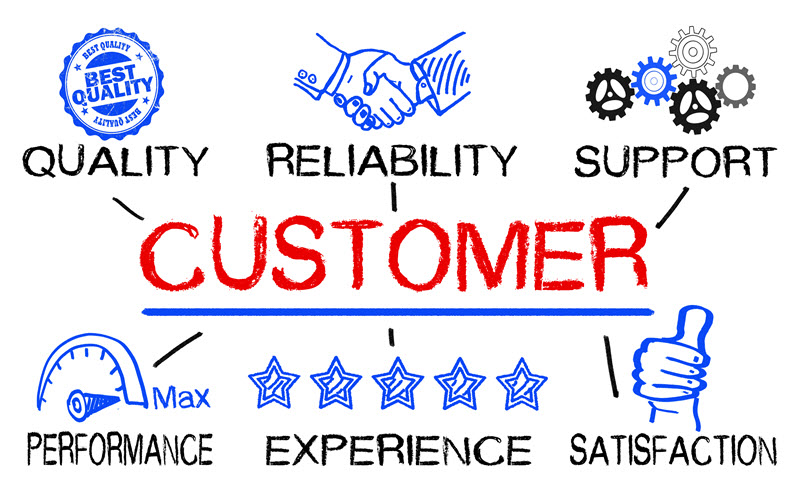
\includegraphics[width=0.8\linewidth]{Customer-Service.jpg}
\end{figure}
\end{frame}

\section{Training and Certification}


\begin{frame}
\frametitle{Training and Certification}
\begin{itemize}
\item<1-> \href{https://training.looker.com/looker-for-data-consumers}{Free Consumer training}
\item<1-> \href{https://verify.skilljar.com/c/3hki2a4qvgok}{Certificate}
\item<2-> \href{https://training.looker.com/looker-for-data-explorers}{Free Data Explorer training}
\item<2-> \href{https://verify.skilljar.com/c/em6yhniy2iee}{Certificate}
\item<3-> \href{https://training.looker.com/looker-development-foundations}{Free LookML Developer training}

\end{itemize}
\end{frame}

%----------------------------------------------------------------------------------------
\section{Q \& A}



\end{document}